
% JuliaCon proceedings template
\documentclass{juliacon}
\setcounter{page}{1}

\begin{document}

% **************GENERATED FILE, DO NOT EDIT**************

\title{BlankLocalizationCore.jl: implementing blank localization in Julia}

\author[1, 2]{Tamás Cserteg}
\author[1]{András Kovács}
\author[1, 3]{József Váncza}
\affil[1]{EPIC Centre of Excellence, HUN-REN Institute for Computer Science and Control (SZTAKI), Budapest H-1111, Hungary}
\affil[2]{Doctoral School of Informatics, ELTE Eötvös Loránd University, Budapest H-1117, Hungary}
\affil[3]{Department of Manufacturing Science and Technology, Budapest University of Technology and Economics, Budapest H-1111, Hungary}

\keywords{Julia, Optimization, Machining, Blank localization}

\hypersetup{
pdftitle = {BlankLocalizationCore.jl: implementing blank localization in Julia},
pdfsubject = {JuliaCon 2022 Proceedings},
pdfauthor = {Tamás Cserteg, András Kovács, József Váncza},
pdfkeywords = {Julia, Optimization, Machining, Blank localization},
}


%TODO: ha kell hely, akkor Jóska BME-t törölhetjük

\maketitle

\begin{abstract}

Blank localization (also known as workpiece referencing) is an essential task in machining.
It aims to precisely establish the geometric relation of the machine tool (mill, lathe, etc.) and the workpiece.
We introduced the concept of multi-operation blank localization to address this task for drilling and milling scenarios in a semi-automated way,
%TODO: innentől a mondat második fele cut?
which allows positioning different machining features (e.g., different holes) separately in order to exploit the tolerances on the relative position of those features to compensate the small errors of the blank.
The method takes as input the measured rough geometry and the machining CNC code, and computes the best possible position of each feature considering machining allowances and tolerances by solving a convex quadratically constrained quadratic program (QCQP).
The versatility and extensibility of the Julia language helped the development of this algorithm, materializing in the \texttt{BlankLocalizationCore.jl} package.
Its flexibility and ease of use make it an excellent research tool that can be deployed in production as well.
\end{abstract}

\section{Introduction}
\label{sec:intro}
Cast parts may have small geometric variations from lot to lot that need to be addressed before machining by altering the CNC code.
Current practice is dominated by iterative adjustments by human operators, which requires highly trained workers and takes a long time.
%, and still, may produce scrap.
%TODO: kell egyáltalán ezeket hivatkozni?
Automated methods exist for complex free-form parts like wind turbines that place the entire blank as a single solid object \cite{ding:2021_CoarsefineOptimizationMethod}\cite{tan:2014_UnconstrainedApproachBlank}.
Multi-operation blank localization~\cite{cserteg:2023_Annals} however handles group of features independently providing greater flexibility than traditional approaches.
It focuses on drilling and milling which are among the most common machining operations, making it applicable to a wide range of products.
The abstract method and its implementation were developed in parallel, which required a language with wide variety of tools and support for easy prototyping.
Exactly for these reasons we chose the Julia language~\cite{bezanson2017julia}.

\section{Multi-operation blank localization}
\label{sec:algo}

The problem involves looking for the optimal position for each to-be-machined feature (short: machined feature) on the workpiece.
%chatgpt
These features are grouped together, with each group defined relative to a specific reference point known as the part zero.
The layout of these part zeros is controlled by the structure of the machining CNC code.
By moving the part zeros, we can indirectly control the positions of the associated features.
Each part zero—and by extension, each group—can be moved independently, which gives the method its flexibility.
In the optimization program, the positions of the part zeros are the decision variables.

%eredeti
\iffalse
These features are structured into groups, each group being defined relative to a common reference, called part zero.
This is defined by the structure of the machining CNC code.
This means that we can influence the features' positions through moving the part zeros.
Part zeros (thus the groups) can be moved separately, which gives the method its flexibility.
The position of the part zeros are the decision variables of the optimization program.
\fi
%Features within the same group must be moved together, but different feature groups can be moved separately.
%TODO: optimalizáló leírás:
% 0. motiváció
% 1. mik a döntések
% 2. mik a korlátok
% 3. mi a célfv

The machined features need to "enclose" the pre-cast features on the blank (called rough features) with a minimum machining allowance which ensures the required surface finish.
The allowance calculation requires the final part specification in the form of the machining CNC code as well as a representation of the rough geometries.
From their positions and geometric parameters their distance can be computed, which then can be used to generate the allowance constraints for the optimization program.

The other set of constraints roots from respecting the dimensional tolerances describing functional properties (e.g. connections to mating parts).
The developed tolerance model encodes the distance of machined-machined (or sometimes machined-rough) features as axis-aligned minimum and maximum distance.
%These distances form constraints in the optimization program, while minimizing the deviation relative to their mean (central?) value across all tolerances is the objective function itself.
Fig.~\ref{fig:hatfig} from \cite{cserteg:2023_Annals} shows some examples for these features.

\begin{figure}[b]
	\centerline{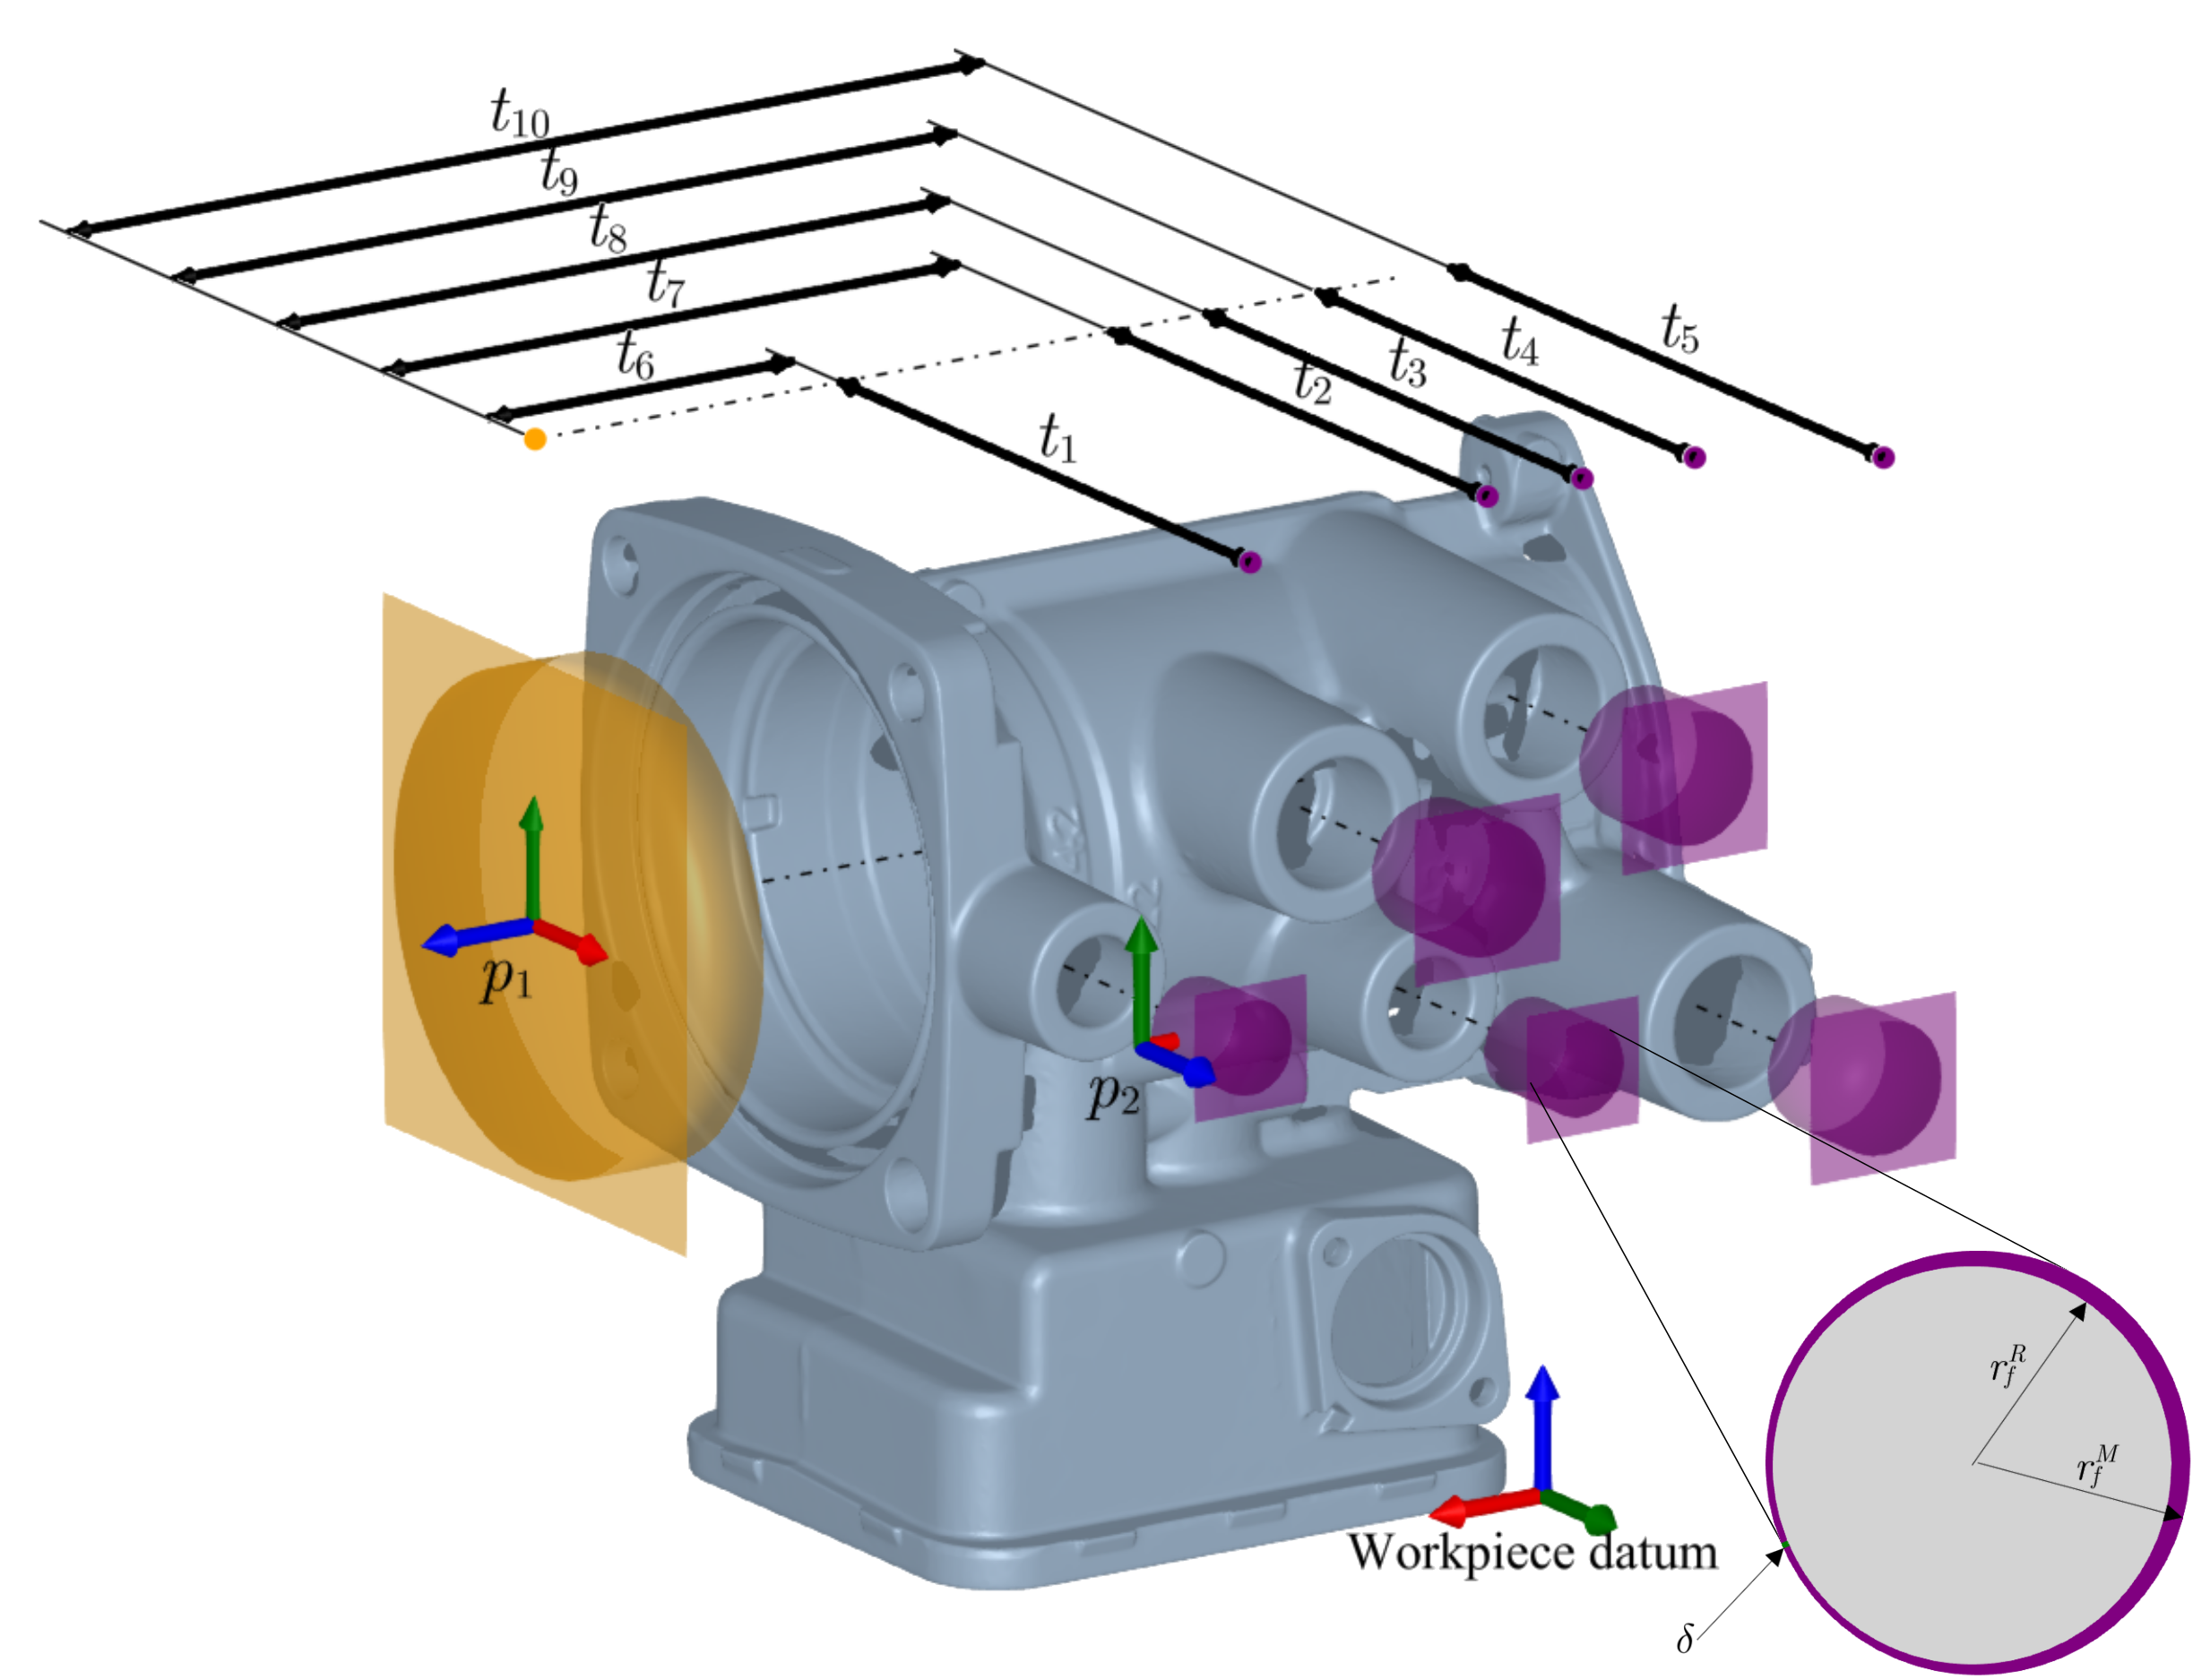
\includegraphics[width=0.95\columnwidth]{cirp-annals-2023-figure-2.png}}
	\caption{3D scanned rough features (in grey), two machined feature groups (orange and purple) with their part zeros, and tolerances connecting the machined features~\cite{cserteg:2023_Annals}.}
	%\caption{Measured part with two machined feature groups and tolerances between them. $r^M$ and $r^R$ denote the machined and rough radii of a feature, while $\delta$ the machining allowance \cite{cserteg:2023_Annals}.}
	\label{fig:hatfig}
\end{figure}

%A tolerance model was developed to replicate the tolerances used in design and machining process.



% vagy full stop, vagy "while ensuring the above constraints are respected
Following common machining practice, the objective of the optimization program is to achieve as little tolerance deviation as possible.
The problem is formulated as a convex quadratically constrained quadratic program (convex QCQP).
%, where decision variables are the positions of the part zeros.
%TODO az hogy a part zeroval mozgatunk, az legyen tisztázva korábban
%The features are moved through their part zeros, which are the variables of the developed .
The optimization model itself and use-cases are described in \cite{cserteg:2023_CMS} and \cite{cserteg:2023_Annals}, while implementation details are given in the following section.

%These feature points can be a point of a plane or the center point of the end face of a cylinder for example.
%The former encodes the requirement that material needs to be removed to ensure proper surface finish and is described for a feature as the smallest thickness of removed material.
%A dimensional tolerance between two features is modeled as lower and upper bounds on the distance between the two features.
%As feature groups move together, only inter-group tolerances need to be considered.


%Briefly we can summarize the multi-operation blank localization as a method that aligns the machined and rough geometries with the required minimum overlap.
%It does it while making sure that features that are connected by dimensional tolerances are within the required distance range.

%Tolerance model is used
%Geometric computations
%Those two are bundled in a convex optimization problem.

%TODO: kihagyni a feature pontokat egy az egyben: Distance of freatures
%mi a feladat és milyen követelményeket támaszt az implementáció felé
% előbb feladatról beszélni és utána julia implementáció követeleményekről?
%todo: deklaratív megoldás
% feladat specifikáció: rough leírás, megmunkálandó leírás, toleranciák (alkatrészrajz, cnc kód)
% ebből a sokféle adatból készül a modell
%modellépítés: összes korlátot és célfv-t definiálni kell és annak az összes paraméterét ki kell számolni
% a geometriai számítűsok ahhoz kellenek, hogy kigeneráljuk a modell egyenleteit, amiknek önmagukban nincs jelentésük, mert csak egyenlőtlenségek.
%megoldás: darál a solver. Nem csinálunk semmit. - tök általános célú QCQP solver, aminek az eredményét valahogy implementálni kell
% kimenteni a part zerokat, és kiértékelni, hogy tolerancia ígyúgy, allownace ezaz meg vizualizáció

%todo az absztrakt modellépítést implementálja a julia implementáció sokkal részletesebben
% modellépítés és instancia generálás
% modellépítés, mint adatokkal való feltöltés <- ezt a julia csinálja
%The tolerance evaluation is part of the objective of the optimization model which means that the distance of these features needs to be often calculated.
%The distance of these features points, thus the evaluation of the tolerance depends on the position of these features which means that the tolerance values need to be evaluated while solving the optimization model.

%Evaluating the minimum machining allowance contributes to the constraints of the optimization program and depends on geometric calculations as well.
%The allowance calculation requires the position of the features as well as other geometric parameter (radii of cylinders for example).

%While an appropriate solver is needed for this family of problems, the solver also needs to evaluate the above described tolerance model and geometric queries during solution.
%We detail this interaction in the next section, while the algorithm itself is described in \cite{cserteg:2023_CMS} and \cite{cserteg:2023_Annals}.

\section{Implementation in Julia}
\label{sec:approach}

%The following aspects of julia enabled us to develop the model and its implementation quickly and efficiently
%During the development of the algorithm, the following requirements were formulated::
%we needed a software tool that supports the quick prototyping needs of research, while giving a solid foundation to validate the concept with our industry partner.
%Summarizin
%Julia helped us to develop the implementation that had the following properties

%The implementation needed to be ilyen, which 
Julia enabled us to develop an implementation with the following properties:
\begin{itemize}
	%TODO: vagy legyen két rész a rapid prototypinggal vagy skip
	\item Concise interface to generate the parameters of the declarative optimization program based on procedural geometric calculations.
%	\item Interfaces our model to the optimization solver and enables rapid prototyping.
	\item Support for a variety of geometrical representations, especially regarding the differences of drilling/milling operations and free-form/primitive geometry representations.
	\item Support for analyzing and visualizing the results.
\end{itemize}

%TODO: asbtract type system is a good base for handling the import fnctions for the measuremnt tool

The heart of the implementation is the solver provided by the JuMP ecosystem~\cite{Lubin2023}.
With JuMP's excellent design, combining the necessary geometric calculations and the declarative optimization program definition was straightforward.
%implementing the optimization model was as easy as repeating the mathematical model in Julia.
%TODO
%jjumps support for declarative programming meets with julia's abstract type system and procedural techniques for geometrical computations
% az együtthatókat könnyű volt juliaból generálni, mert absztrakt módon könnyű megkeresni őket (vagy mi)
Other advantage of JuMP is that solvers can be easily swapped.
For development, the (commercial) FICO Xpress solver was used, but our industry partner could use the (open source) Ipopt or SCIP solvers without issue.

%TODO: absztrakt typusokra deinfinájuk a funckiókat, amiket aztán alacsony sznten könnyű implementálni

%TODO: azt kell elmagyarázni, hogy különböző geometria reprezentációk vannak különböző mérésekből
% de nekünk mindig ugyanaz az információ: a feature point kell
% és ezzel az interfésszel mindenféle mérőeszköz formátumát le tudjuk kezelni
% és van egy egységes interface a feautre pointok (geometriaia leírók, paraméterek?) lekérdezéséhez

To handle the tolerance and allowance calculations, the part definition (CNC code), rough geometry measurements and tolerances need to be stored.
Their representation is built upon a flexible geometry type system.
%To generate the optimization model we needed to store the 1. nc code 2. rough geometry 3. tolerances.
%A common thing regarding the first two, that some kind of geometric representation is needed.

The CNC code can be represented with plane and cylinder geometries for milling and drilling operations.
This "type" information of the geometries is encoded with Julia types.
The primitive or free-form nature of the geometries is implemented with the holy traits pattern and is necessary because different instruments output different types of geometric data.
For example, a coordinate measurement machine will provide primitive geometry definitions like disks and cylinders, while a 3D scanner outputs point clouds or meshes (called free-form collectively).
The \texttt{IsPrimitve} or \texttt{IsFreeForm} traits are applied to geometry types independently of their planar or cylindrical type.
Code block~\ref{lst:def-types} shows a shortened version of the implemented type system.

\begin{lstlisting}[language = Julia, numbers=left, label={lst:def-types}, caption={Shortened implementation of the type system used by \texttt{BlankLocalizationCore.jl}.}]
# Type tree for localization geometries.
# "ALoc": AbstractLocalization
abstract type ALocGeometry end
abstract type AHoleGeometry <: ALocGeometry end
abstract type APlaneGeometry <: ALocGeometry end

# Trait to describe the "style" of an ALocGeometry.
abstract type GeometryStyle end
struct IsPrimitive <: GeometryStyle end
struct IsFreeForm <: GeometryStyle end
\end{lstlisting}

The optimization model uses a "feature point" concept which requires the position and some parameters of the geometries.
A function interface is designed for accessing these values.
%is that it is built around "feature points" (consistently defined points of different geometries).
%The other part of the optimization generation interface is definition of the query functions that work on these types.
The package documentation contains the list of functions that need to be defined but some are showcased in code block~\ref{lst:example}.
%Free form geometries need to implement the \texttt{surfacepoints} and \texttt{filteredsurfacepoints} methods;
%Primitive geometries need to have the \texttt{featurepoint} method and cylindrical features need the \texttt{featureradius} on top of that.
One function that we want to highlight is the \texttt{visualizationgeometry}, which needs to return a \texttt{Meshes.jl} object that will be passed to the \texttt{Meshes.viz} function.
%The visulization interface is built around Meshes.jl, therefore the to-be-showed geometries must be from that package.
Using the Meshes ecosystem~\cite{Hoffimann2023}, we could not only interactively inspect the results of the optimization, but also produce publication quality images, like Fig.~\ref{fig:hatfig} in \cite{cserteg:2023_Annals}.

\vspace*{2em}

\begin{lstlisting}[language = Julia, numbers=left, label={lst:example}, caption={Defining a new type for the optimization model.}]
struct MyDisk <: AHoleGeometry
  p::Vector{Float64} # center point
  n::Vector{Float64} # surface normal
  d::Float64 # diameter
end

GeometryStyle(::Type{MyDisk}) = IsPrimitive()

featurepoint(::IsPrimitive, x::MyDisk) = x.p
featureradius(::IsPrimitive, x::MyDisk) = x.d/2

using Meshes

function visualizationgeometry(geom::MyDisk)
  plane = Plane(Point3(geom.p), Vec3(geom.n))
  return Disk(plane, geom.d/2)
end
\end{lstlisting}


\iffalse
The optimization program uses a feature point (or feature points for free-form geometries) of features, that is used for computing the machining allowance and the dimensional tolerances.
A function interface is defined for querying these feature points of geometries, that is used to generate the optimization program.
Code block~\ref{lst:example} shows the definition of those functions as well.
The visulization interface is built around Meshes.jl, therefore the to-be-showed geometries must be from that package.
Using the Meshes ecosystem, we could produce publication quality images, like Fig.~\ref{fig:hatfig} from \cite{cserteg:2023_Annals}.


The optimization generation engine uses the functions defined by this interface to construct the optimization program.

As mentioned earlier, an important requirement was to handle the output formats of many different devices.
Every measurement instrument comes with its own processing software and export formats, not necessarily designed for interoperability.
As a result, we needed to write (or use) parsers for different text and tabular formats.
\fi

\section{Results and future work}
\label{sec:results}
%TODO
Future plans for the package and the method itself include an overhaul of the tolerance modeling scheme.
Currently, only dimensional tolerances are handled, but it should be discovered if more GD\&T tolerances can be incorporated into the model.
The current implementation supports only cylinders and planes, thus drilling and milling; it is a future research direction to extend the handled machining operations, e.g., to turning.

\section{Acknowledgments}
The research was supported by the European Union within the framework of the National Laboratory for Autonomous Systems (RRF-2.3.1-21-2022-00002) and the TKP2021-NKTA-01  NRDIO grant on "Research on cooperative production and logistics systems to support a competitive and sustainable economy".

% **************GENERATED FILE, DO NOT EDIT**************

\bibliographystyle{juliacon}
\bibliography{ref.bib}


\end{document}

% Inspired by the International Journal of Computer Applications template
